% Chapter 14: protein structure prediction with AlphaFold 2.
% Requires: amsmath, amssymb, bm, graphicx, booktabs, multirow, subcaption, algorithm, algpseudocode,
% tikz (arrows.meta, positioning, calc, decorations.pathreplacing, decorations.pathmorphing, shapes.geometric, fit), natbib.
% Computed figures are produced by scripts/make_figures.py; figures/slides/ holds figures taken from the lecture slides.

\providecommand{\R}{\mathbb{R}}
\providecommand{\E}{\mathbb{E}}
\providecommand{\Normal}{\mathcal{N}}
\providecommand{\argmax}{\operatorname*{arg\,max}}
\providecommand{\argmin}{\operatorname*{arg\,min}}
\providecommand{\vy}{\mathbf{y}}
\providecommand{\vx}{\mathbf{x}}
\providecommand{\mX}{\mathbf{X}}
\providecommand{\mI}{\mathbf{I}}
\providecommand{\vb}{\boldsymbol{\beta}}
\providecommand{\veps}{\boldsymbol{\epsilon}}
\providecommand{\vp}{\mathbf{p}}
\providecommand{\vg}{\mathbf{g}}
\providecommand{\ind}{\mathbf{1}}
\providecommand{\vh}{\mathbf{h}}
\providecommand{\vq}{\mathbf{q}}
\providecommand{\vk}{\mathbf{k}}
\providecommand{\vv}{\mathbf{v}}
\providecommand{\vz}{\mathbf{z}}
\providecommand{\ve}{\mathbf{e}}
\providecommand{\va}{\mathbf{a}}
\providecommand{\vs}{\mathbf{s}}
\providecommand{\mW}{\mathbf{W}}
\providecommand{\mR}{\mathbf{R}}
\providecommand{\softmax}{\operatorname{softmax}}
\providecommand{\vm}{\mathbf{m}}
\providecommand{\vo}{\mathbf{o}}
\providecommand{\vt}{\mathbf{t}}
\providecommand{\vu}{\mathbf{u}}
\providecommand{\vw}{\mathbf{w}}
\providecommand{\vc}{\mathbf{c}}
\providecommand{\vf}{\mathbf{f}}
\providecommand{\mF}{\mathbf{F}}
\providecommand{\mM}{\mathbf{M}}
\providecommand{\mJ}{\mathbf{J}}
\providecommand{\SE}{\mathrm{SE}(3)}
\providecommand{\SO}{\mathrm{SO}(3)}
\providecommand{\LN}{\operatorname{LN}}
\providecommand{\sigm}{\operatorname{sigmoid}}
\providecommand{\Ca}{C$\alpha$}

\providecommand{\chaptertoc}{}
\chapter{Protein structure prediction with AlphaFold~2}
\label{ch:alphafold}
\chaptertoc

A protein is a chain of amino acids that folds into a three-dimensional shape, and that shape determines what the protein does. Measuring the shape experimentally takes months or years per protein, while sequencing gives us the amino acid sequences of millions of proteins cheaply. Predicting structure from sequence has therefore been a central problem of computational biology for half a century. AlphaFold~2~\citep{jumper2021} solved a large part of this problem in 2020, predicting the structures of many proteins with an accuracy close to that of experiment. It has had a large influence on the interface of machine learning and biology, and its main ideas recur in later models.

AlphaFold~2 combines ideas we have met in earlier chapters, attention and transformers (Chapter 3) and representation learning from large data sets, with ideas specific to proteins. This chapter covers four of these. The first is \emph{evolutionary information}: related proteins in other species, lined up in a multiple sequence alignment, reveal which positions of a protein are in contact. The second is the \emph{Evoformer}, a transformer that operates on two coupled representations, one of the alignment and one of pairs of residues, and that is built to respect the geometry of distances. The third is the \emph{structure module}, which places each residue in space as a rigid body and is designed so that its predictions rotate and translate with the protein. The fourth is the training objective, in particular a loss that compares structures without first superimposing them, and the model's prediction of its own confidence. The presentation follows \citet{jumper2021} and the expository account of \citet{bouatta2021}; the supplementary information of \citet{jumper2021} gives every layer in pseudocode.

%======================================================================
\section{Proteins and the structure prediction problem}
\label{sec:proteins}
%======================================================================

\subsection{Amino acids, the backbone and side chains}

Chapter 1 introduced the central dogma: DNA is transcribed to RNA, which is translated into protein. Translation reads the RNA three nucleotides (one codon) at a time and appends one of 20 amino acids for each codon, so a protein is a linear polymer, a sequence over an alphabet of 20 letters. In the context of a protein, each amino acid is called a \emph{residue}. Typical proteins are a few hundred residues long.

Every amino acid shares the same core of atoms: a nitrogen (N), a central carbon called the alpha carbon (\Ca) and a carbonyl carbon (C, sometimes written C$'$) bonded to an oxygen. Consecutive residues are joined by a \emph{peptide bond} between the carbonyl carbon of one residue and the nitrogen of the next. The repeating chain N--\Ca--C--N--\Ca--C--$\cdots$ is the \emph{backbone} (Figure~\ref{fig:backbone}). What distinguishes the 20 amino acids is the \emph{side chain} attached to the \Ca, which ranges from a single hydrogen (glycine) to large ring structures (tryptophan), and which can be hydrophobic, charged or polar.

The backbone is not rigid. Bond lengths and bond angles are nearly fixed, so the conformation of the backbone is described by three \emph{torsion} (dihedral) angles per residue: $\phi$ about the N--\Ca{} bond, $\psi$ about the \Ca--C bond and $\omega$ about the peptide bond. The peptide bond has partial double-bond character, so $\omega$ is close to $180^\circ$ in almost all residues. Not all combinations of $\phi$ and $\psi$ are possible, because some would make atoms collide; the allowed regions of the $(\phi,\psi)$ plane form the Ramachandran plot~\citep{ramachandran1963}. Repeating patterns of $(\phi,\psi)$ give the regular \emph{secondary structures}, the $\alpha$-helix and the $\beta$-strand. Side chains have up to four further torsion angles, $\chi_1,\dots,\chi_4$, that set their conformation.

\begin{figure}[!htbp]
  \centering
  \begin{tikzpicture}[>=Stealth, every node/.style={font=\small},
      atom/.style={circle, draw, inner sep=1.2pt, minimum size=5mm},
      tri/.style={fill=red!15, draw=red!70!black, thick}]
    % three residues in a zig-zag
    \foreach \r/\x in {1/0, 2/4.2, 3/8.4} {
      \coordinate (N\r) at (\x,0);
      \coordinate (A\r) at (\x+1.2,0.8);
      \coordinate (C\r) at (\x+2.6,0.2);
      \fill[tri] (N\r) -- (A\r) -- (C\r) -- cycle;
    }
    \draw[thick] (C1) -- (N2); \draw[thick] (C2) -- (N3);
    \foreach \r in {1,2,3} {
      \draw[thick] (N\r) -- (A\r) -- (C\r);
      \draw[thick] (C\r) -- ++(0.15,-1.0) coordinate (O\r);
      \draw[thick] (A\r) -- ++(0,1.0) coordinate (S\r);
      \node[atom, fill=blue!25] at (N\r) {N};
      \node[atom, fill=gray!30] at (A\r) {\scriptsize C$\alpha$};
      \node[atom, fill=gray!60] at (C\r) {C};
      \node[atom, fill=red!40] at (O\r) {O};
      \node[draw, rounded corners, fill=orange!30, inner sep=2pt] at (S\r) {R$_\r$};
    }
    \draw[gray] ($(C1)!0.5!(N2)$) -- (3.25,-0.45) node[right, font=\footnotesize] {peptide bond};
    % torsion labels for residue 2
    \draw[->, blue!60!black] ($(N2)!0.5!(A2)+(-0.35,0.35)$) arc[start angle=150, end angle=390, x radius=0.22, y radius=0.12];
    \node[blue!60!black] at ($(N2)!0.5!(A2)+(-0.55,0.55)$) {$\phi$};
    \draw[->, blue!60!black] ($(A2)!0.5!(C2)+(0.1,0.32)$) arc[start angle=150, end angle=390, x radius=0.22, y radius=0.12];
    \node[blue!60!black] at ($(A2)!0.5!(C2)+(0.1,0.65)$) {$\psi$};
    \draw[->, blue!60!black] ($(C2)!0.5!(N3)+(0,0.3)$) arc[start angle=150, end angle=390, x radius=0.22, y radius=0.12];
    \node[blue!60!black] at ($(C2)!0.5!(N3)+(0,0.62)$) {$\omega$};
    \node[orange!60!black, font=\footnotesize, align=center] at (5.4,2.75) {side chain,\\torsions $\chi_1,\dots,\chi_4$};
    \draw[decorate, decoration={brace, mirror, amplitude=4pt}] (4.0,-1.35) -- (7.0,-1.35) node[midway, below=4pt, font=\footnotesize] {residue $i$};
    \node[left] at (-0.3,0) {$\cdots$}; \node[right] at (11.3,0.2) {$\cdots$};
  \end{tikzpicture}
  \caption{Three residues of a protein backbone. Each residue contributes N, \Ca{} and C atoms to the backbone and carries a side chain R$_i$ on its \Ca. The backbone conformation is set by the torsion angles $\phi$, $\psi$ and $\omega$ (shown for the middle residue), and each side chain by up to four further torsions. AlphaFold~2 represents each residue by the rigid triangle of its N, \Ca{} and C atoms (shaded).}
  \label{fig:backbone}
\end{figure}

\subsection{Why structure, and where the data come from}

The sequence of a protein determines its structure, at least for proteins that fold on their own: an unfolded protein in solution refolds into its native shape~\citep{anfinsen1973}. The structure in turn determines function. An enzyme's active site is a pocket in which a few residues, often far apart in the sequence, are brought together; a receptor binds its ligand through a surface whose shape and charge match it. Knowing the structure of a protein helps to design drugs that bind it, to interpret the effects of mutations (which we met as genetic variants in earlier chapters), and to engineer new proteins.

Structures are determined experimentally, mostly by X-ray crystallography, nuclear magnetic resonance and, increasingly, cryo-electron microscopy. Crystallography requires coaxing the protein to form a crystal, which can take years for a single protein. The Protein Data Bank (PDB) collects the results: around 200,000 structures from about five decades of work. This is the training data that made AlphaFold possible. Every component of the model had earlier work behind it; much of the advance was in combining these components and training them together on this data.

\subsection{The prediction problem}

The input to AlphaFold~2 is a single amino acid sequence of length $R$ (the number of residues). The output is the three-dimensional coordinates of every heavy atom of the protein, together with a per-residue confidence. Low confidence does not only reflect a lack of training data. Some regions of proteins are \emph{intrinsically disordered}: they do not adopt a single structure but move between many conformations, and no single prediction can be correct for them. A useful confidence measure flags these regions.

Two properties of the problem shape the model. First, a structure has no preferred position or orientation: rotating or translating a protein does not change it. The model's output should rotate and translate with any rotation or translation of its internal coordinates, and the loss should not depend on them. Second, the information in a single sequence is limited; most of the signal AlphaFold uses comes from related sequences, which we turn to next.

%======================================================================
\section{Evolutionary information}
\label{sec:evolution}
%======================================================================

\subsection{Homologs and multiple sequence alignments}

New genes arise mostly by duplication of existing genes followed by divergence, and genes are passed from ancestral species to their descendants. Genes that share a common ancestor are \emph{homologs}. Homologs in different species, such as human and mouse haemoglobin $\beta$, are \emph{orthologs}; homologs within the same species, such as human haemoglobin $\alpha$ and $\beta$, are \emph{paralogs}. Homologous proteins usually have similar structures even when their sequences have diverged considerably, because structure is under stronger selection than sequence.

AlphaFold's first step is a \emph{genetic database search}: it searches large protein sequence databases, built from sequenced genomes and metagenomes, for homologs of the input sequence. The homologs are lined up in a \emph{multiple sequence alignment} (MSA) in which each row is one sequence and each column corresponds to one position of the input (the \emph{target}) sequence (Figure~\ref{fig:msa_cartoon}). Insertions relative to the target are removed and deletions are marked with a gap symbol, so the MSA is an $S\times R$ array over 21 symbols, where $S$ is the number of sequences. The target sequence is the first row. Deep MSAs, with thousands of diverse sequences, are available for well-studied protein families; some proteins, called orphans, have few or no detectable homologs.

\begin{figure}[!htbp]
  \centering
  \begin{tikzpicture}[>=Stealth, every node/.style={font=\small}]
    % columns of the alignment (one list per column, top row = target)
    \foreach \col [count=\i] in {{A,A,G,G,A,G},{R,R,K,K,R,R},{P,P,P,P,P,A},{C,C,C,C,C,C},{L,I,L,I,L,V},{V,V,V,I,V,V},{D,D,E,E,D,D},{S,C,S,S,S,A},{Q,N,H,D,A,T}} {
      \foreach \c [count=\s] in \col {
        \node[font=\ttfamily\small, minimum width=0.5cm, minimum height=0.45cm, inner sep=0pt] at (0.55*\i, -0.45*\s) {\c};
      }
    }
    \draw[thick, red!70!black, rounded corners=2pt] (0.55*2-0.25,-0.2) rectangle (0.55*2+0.25,-2.92);
    \draw[thick, red!70!black, rounded corners=2pt] (0.55*7-0.25,-0.2) rectangle (0.55*7+0.25,-2.92);
    \draw[thick, blue!60!black, rounded corners=2pt] (0.55*4-0.25,-0.2) rectangle (0.55*4+0.25,-2.92);
    \draw[thick, green!50!black, rounded corners=2pt] (0.55*9-0.25,-0.2) rectangle (0.55*9+0.25,-2.92);
    \draw[red!70!black] (0.55*2,0.0) -- (0.55*2,0.25) -- node[above, font=\footnotesize] {co-evolving} (0.55*7,0.25) -- (0.55*7,0.0);
    \node[blue!60!black, font=\footnotesize, align=center] at (0.55*4,-3.45) {conserved};
    \node[green!50!black, font=\footnotesize, align=center] at (0.55*9+0.15,-3.45) {variable};
    \node[left, font=\footnotesize] at (0.2,-0.45) {target};
    \draw[decorate, decoration={brace, amplitude=4pt}] (0.05,-2.85) -- (0.05,-0.7) node[midway, left=5pt, font=\footnotesize, align=right] {homologs};
    % folded chain with the two co-evolving positions in contact
    \begin{scope}[xshift=7.6cm, yshift=-1.5cm]
      \coordinate (p1) at (-1.6,-0.9); \coordinate (p2) at (-0.9,-0.3); \coordinate (p3) at (-1.2,0.6);
      \coordinate (p4) at (-0.3,1.2); \coordinate (p5) at (0.6,0.9); \coordinate (p6) at (1.0,0.0);
      \coordinate (p7) at (0.0,-0.35); \coordinate (p8) at (0.5,-1.1); \coordinate (p9) at (1.4,-1.3);
      \draw[thick, gray] (p1) \foreach \k in {2,...,9} { -- (p\k) };
      \foreach \k in {1,...,9} \fill[gray!60] (p\k) circle (0.13);
      \fill[blue!60!black] (p4) circle (0.15);
      \fill[red!70!black] (p2) circle (0.16); \fill[red!70!black] (p7) circle (0.16);
      \draw[red!70!black, dashed, thick] (p2) -- (p7);
      \node[red!70!black, font=\footnotesize] at (-0.45,-0.75) {contact};
      \node[font=\footnotesize] at (p2) [above left] {2};
      \node[font=\footnotesize] at (p7) [below right] {7};
    \end{scope}
  \end{tikzpicture}
  \caption{A toy multiple sequence alignment. Each row is a homolog of the target sequence (top row) and each column an aligned position. Position 4 is conserved; position 9 varies freely. Positions 2 and 7 co-evolve: wherever position 2 has R, position 7 has D, and wherever position 2 has K, position 7 has E. A positive residue at one position is always paired with a negative residue at the other, as expected if the two form a salt bridge. Positions that co-evolve are often in contact in the folded structure (right), even when they are far apart in the sequence. After a slide adapted from M.~AlQuraishi.}
  \label{fig:msa_cartoon}
\end{figure}

\subsection{Conservation and coevolution}

An MSA carries two kinds of information about structure. The first is in single columns. A \emph{conserved} column, where almost every homolog has the same residue, marks a position under strong selection, often one that is buried in the core of the protein or that takes part in its function. The second is in pairs of columns. Suppose residues $i$ and $j$ are in contact in the folded structure, for example a positive and a negative residue forming a salt bridge. A mutation at $i$ that changes its charge breaks the contact and destabilizes the protein, unless a compensating mutation at $j$ restores it. Over evolutionary time, the residues at $i$ and $j$ therefore change together: they \emph{co-evolve}. Detecting co-evolving pairs of columns gives a prediction of which residues are in contact, even when they are far apart in sequence~\citep{gobel1994}. A map of contacts, in turn, constrains the fold.

Let $x_{si}\in\{1,\dots,q\}$ be the symbol of sequence $s$ at position $i$, with $q=21$ for the 20 amino acids and the gap. The single and pair frequencies are
\begin{equation}
  f_i(a) = \frac{1}{S}\sum_{s=1}^S \ind[x_{si}=a], \qquad
  f_{ij}(a,b) = \frac{1}{S}\sum_{s=1}^S \ind[x_{si}=a]\,\ind[x_{sj}=b],
  \label{eq:msa_freqs}
\end{equation}
for $a,b\in\{1,\dots,q\}$, usually computed with a small pseudocount and with sequences reweighted to reduce redundancy. The \emph{mutual information} between columns $i$ and $j$,
\begin{equation}
  \text{MI}_{ij} = \sum_{a=1}^q\sum_{b=1}^q f_{ij}(a,b)\log\frac{f_{ij}(a,b)}{f_i(a)\,f_j(b)},
\end{equation}
is zero when the two columns are independent and positive otherwise. Ranking pairs by MI is the simplest coevolution-based contact predictor. It has two weaknesses. First, the sequences in an MSA are related by a phylogeny: closely related sequences share many residues by descent, not because of structural constraints, and this inflates MI for all pairs of variable columns. A simple fix is the \emph{average product correction} (APC)~\citep{dunn2008},
\begin{equation}
  \text{MI}^{\text{APC}}_{ij} = \text{MI}_{ij} - \frac{\overline{\text{MI}}_{i\cdot}\,\overline{\text{MI}}_{\cdot j}}{\overline{\text{MI}}_{\cdot\cdot}},
\end{equation}
where $\overline{\text{MI}}_{i\cdot}$ is the mean MI of column $i$ with all other columns and $\overline{\text{MI}}_{\cdot\cdot}$ the mean over all pairs. Columns that are correlated with everything, through phylogeny or high variability, are penalized. Second, correlations are transitive: if $i$ contacts $j$ and $j$ contacts $k$, columns $i$ and $k$ are correlated without being in contact. \emph{Direct coupling analysis}~\citep{morcos2011,marks2011} addresses this by fitting a global model to the whole alignment, a Potts model
\begin{equation}
  p(x_1,\dots,x_R) = \frac{1}{Z}\exp\left(\sum_{i=1}^R h_i(x_i) + \sum_{i<j} J_{ij}(x_i,x_j)\right),
  \label{eq:potts}
\end{equation}
with fields $h_i(a)$ that capture conservation, couplings $J_{ij}(a,b)$ that capture direct interactions, and normalizing constant $Z$. The size of the fitted coupling matrix $\mJ_{ij}\in\R^{q\times q}$ predicts contacts. Correlations between $i$ and $k$ that are explained by couplings through $j$ do not need a direct coupling $J_{ik}$.

Figure~\ref{fig:coevolution} illustrates these points on simulated data. We evolved 256 sequences of length 40 down a binary tree, with each branch applying a few rounds of mutation under selection by a Potts model with 12 planted contacts and six strongly conserved positions. Raw MI is dominated by phylogenetic correlation: its 12 highest-scoring pairs include 5 of the true contacts. After APC, 8 of the 12 are true contacts. The conserved positions have low MI with everything, since a column that does not vary cannot covary.

\begin{figure}[!htbp]
  \centering
  \includegraphics[width=\linewidth]{coevolution.pdf}
  \caption{Contact prediction from coevolution on a simulated alignment of 256 sequences and 40 positions, evolved down a binary tree under a Potts model~\eqref{eq:potts} with 12 planted contacts. Left: true contacts. Middle: mutual information between columns, scaled to a maximum of one. Right: mutual information after the average product correction, negative values set to zero. Phylogenetic structure gives every pair of variable columns some mutual information; the correction removes much of it.}
  \label{fig:coevolution}
\end{figure}

\subsection{From contacts to structure}

Coevolution-based contact maps, fed to physics-based folding programs, gave the first accurate predictions of the structures of large protein families from sequence alone~\citep{marks2011}. Deep learning then replaced the statistical models: convolutional networks applied to the pair features of an MSA predicted contacts, and then full \emph{distograms}, probability distributions over the distance between every pair of residues. AlphaFold~1~\citep{senior2020} predicted distograms with a deep residual network and then found a structure by gradient descent on a potential built from them.

A distance map is a strong constraint on structure but not the same thing as a structure. Given exact pairwise distances, the structure is determined only up to rotation, translation and mirror reflection; given noisy or partial distances, there may be no structure that satisfies all of them. AlphaFold~2 differs from its predecessors in predicting the coordinates directly, with a model trained end to end from sequence and MSA to structure~\citep{jumper2021}, an approach also pursued by \citet{alquraishi2019}. Its authors identify this end-to-end training as one of the reasons for its accuracy.

%======================================================================
\section{Overview of AlphaFold~2}
\label{sec:overview}
%======================================================================

Figure~\ref{fig:af2_arch} shows the architecture. Starting from the input sequence, there are three steps.

\begin{enumerate}
  \item \emph{Inputs.} A genetic database search builds an MSA of homologs, and a structure database search finds \emph{templates}, homologs whose structures are in the PDB. Templates are optional; the model works without them. The MSA is embedded as the \emph{MSA representation}, a tensor of shape $S\times R\times D_m$, with one $D_m$-dimensional vector $\vm_{si}$ for each sequence $s$ and residue $i$. Pair features are embedded as the \emph{pair representation}, of shape $R\times R\times D_z$, with one vector $\vz_{ij}$ for each pair of residues. The pair representation is initialized from the target sequence alone (the ``pairing'' step in Figure~\ref{fig:af2_arch}): $\vz_{ij}$ is the sum of a linear embedding of the amino acid at $i$, one of the amino acid at $j$, and an embedding of the sequence separation $j-i$, which acts as a relative positional encoding (Chapter 3). Template structures, when available, add pair features such as the distances between residues in the template.
  \item \emph{Evoformer.} A stack of 48 Evoformer blocks updates the two representations, passing information between them in every block (Section~\ref{sec:evoformer}).
  \item \emph{Structure module.} The first row of the MSA representation, the one for the target sequence, is projected to the \emph{single representation} $\vs_i\in\R^{D_s}$. The structure module, eight blocks with shared weights, uses the single and pair representations to place every residue in space and outputs the coordinates of all atoms and a per-residue confidence (Section~\ref{sec:structure_module}).
\end{enumerate}
The whole network is then run again, three more times at inference, with the outputs of the previous pass added to the inputs of the next: the final pair representation, the first row of the MSA representation and the distances in the predicted structure. This \emph{recycling} lets the network refine its prediction, and acts as a further, shared-weight deepening of an already deep network. Table~\ref{tab:af2_dims} lists the sizes of the representations.

\begin{figure}[!htbp]
  \centering
  \includegraphics[width=\linewidth]{slides/alphafold2_architecture.png}
  \caption{The AlphaFold~2 architecture. The input sequence is used to search genetic and structure databases for an MSA and templates, which initialize the MSA representation ($s\times r\times c$: sequences $\times$ residues $\times$ channels) and the pair representation ($r\times r\times c$). After 48 Evoformer blocks, the single representation (the first row of the MSA representation) and the pair representation are passed to the structure module, which outputs a 3D structure coloured by predicted confidence. The whole network is recycled three times. Reproduced from \citet{jumper2021}.}
  \label{fig:af2_arch}
\end{figure}

\begin{table}[!htbp]
  \centering
  \caption{Representations in AlphaFold~2 and their sizes in the published model~\citep{jumper2021}. $R$ is the number of residues, cropped to at most 384 during training; $S$ is the number of MSA sequences processed by the main Evoformer stack (512 at inference). A further stack of four lighter blocks processes thousands of additional MSA sequences and feeds only the pair representation.}
  \label{tab:af2_dims}
  \begin{tabular}{llll}
    \toprule
    Representation & Element & Shape & Channels \\
    \midrule
    MSA & $\vm_{si}$, sequence $s$, residue $i$ & $S\times R\times D_m$ & $D_m=256$ \\
    Pair & $\vz_{ij}$, residues $i,j$ & $R\times R\times D_z$ & $D_z=128$ \\
    Single & $\vs_i$, residue $i$ & $R\times D_s$ & $D_s=384$ \\
    Backbone frames & $T_i=(\mR_i,\vt_i)$, residue $i$ & $R\times(3\times3+3)$ & -- \\
    \bottomrule
  \end{tabular}
\end{table}

The paper writes $s$, $r$ and $c$ for the numbers of sequences, residues and channels. In this chapter $S$ and $R$ are the numbers of sequences and residues, $s,t$ index sequences, $i,j,k$ index residues, and $D_m$, $D_z$, $D_s$ are channel dimensions.

%======================================================================
\section{Attention with a bias}
\label{sec:attention_recap}
%======================================================================

AlphaFold~2 contains no convolutions. Apart from position-wise linear layers and multilayer perceptrons, all of its layers are variants of attention~\citep{vaswani2017}. We use the notation of Chapter 3. For positions $i,j\in\{1,\dots,L\}$ with representations $\vh_i,\vh_j\in\R^D$, the query, key and value are $\vq_i=\mW^Q\vh_i\in\R^P$, $\vk_j=\mW^K\vh_j\in\R^P$ and $\vv_j=\mW^V\vh_j\in\R^{D_v}$, position $i$ attends to position $j$ with weight
\begin{equation}
  a_{ij} = \softmax_j\left(\frac{\vq_i^\top\vk_j}{\sqrt{P}} + b_{ij}\right) = \frac{\exp\left(\vq_i^\top\vk_j/\sqrt{P} + b_{ij}\right)}{\sum_{j'=1}^L\exp\left(\vq_i^\top\vk_{j'}/\sqrt{P} + b_{ij'}\right)},
  \label{eq:biased_attention}
\end{equation}
and its output is $\vg_i=\sum_j a_{ij}\vv_j$. Compared with Chapter 3 there is one new term, a scalar \emph{bias} $b_{ij}$ added to the score of each pair before the softmax. A positive bias makes $i$ attend more to $j$ whatever their queries and keys say, and a large negative bias forbids it. In Chapter 3 relative positional encodings could enter attention as a bias of this form, depending only on $j-i$; in AlphaFold the bias is computed from the pair representation and so carries the network's current belief about how residues $i$ and $j$ are related.

Two further details recur. AlphaFold uses multi-head attention throughout, with $M$ heads indexed by $m$, each with its own projections and bias. And most attention layers are \emph{gated}: the output of each head is multiplied elementwise by a gate $\sigm(\mW^G\vh_i)\in(0,1)^{D_v}$ computed from the input, which lets each position switch off the update from attention. Each layer is wrapped in layer normalization and a residual connection, as in the transformer block of Chapter 3. To keep the equations short we omit gating, layer normalization and bias vectors of linear layers below unless they matter for the argument; the supplementary information of \citet{jumper2021} gives them all.

%======================================================================
\section{The Evoformer}
\label{sec:evoformer}
%======================================================================

The Evoformer turns the raw MSA and pair features into representations from which a structure can be read off. Its design follows from three questions. How can attention be applied to a two-dimensional array of sequences by positions at a tolerable cost? How should information pass between the MSA and the pair representations? And how can the pair representation be encouraged to behave like a description of geometry? Figure~\ref{fig:evoformer_schematic} summarizes the answers.

\begin{figure}[!htbp]
  \centering
  \begin{tikzpicture}[>=Stealth, every node/.style={font=\small}]
    \pgfmathsetseed{14}
    % MSA representation: S x R grid
    \begin{scope}
      \fill[green!55!black!35] (-0.15,-0.15) rectangle (4.35,2.55);
      \foreach \i in {0,...,8} \foreach \s in {0,...,5} {
        \pgfmathsetmacro{\v}{20+60*rnd}
        \fill[green!\v!yellow] (0.5*\i,0.4*\s) rectangle ++(0.46,0.36);
      }
      \draw[very thick, red!80!black] (-0.05,1.57) rectangle (4.5,1.99);
      \draw[very thick, orange!90!black] (2.96,-0.08) rectangle (3.42,2.48);
      \node[above, align=center] at (2.1,2.6) {MSA representation, $S\times R\times D_m$\\ \footnotesize columns: residues $i$};
      \node[red!80!black, right] at (4.55,1.78) {row attention};
      \node[orange!90!black, below] at (3.19,-0.15) {column attention};
      \draw[decorate, decoration={brace, amplitude=4pt}] (-0.3,0) -- (-0.3,2.36) node[midway, left=5pt] {sequences $s$};
    \end{scope}
    % pair representation: R x R grid
    \begin{scope}[yshift=-6.0cm]
      \fill[blue!45] (-0.15,-0.15) rectangle (4.35,4.65);
      \foreach \i in {0,...,8} \foreach \j in {0,...,8} {
        \pgfmathsetmacro{\v}{15+60*rnd}
        \fill[green!\v!teal!70!black] (0.5*\i,0.5*\j) rectangle ++(0.46,0.46);
      }
      \node[below] at (2.1,-0.2) {pair representation, $R\times R\times D_z$};
      \draw[very thick, red!80!black] (2.46,2.96) rectangle (2.96,3.46);
      \node[white, font=\footnotesize] at (2.71,3.21) {$ij$};
      \draw[decorate, decoration={brace, mirror, amplitude=4pt}] (-0.3,4.5) -- (-0.3,0) node[midway, left=5pt] {residues $i$};
    \end{scope}
    % arrows between tracks
    \draw[->, very thick, blue!60!black] (1.0,-1.35) -- node[left, align=right, font=\footnotesize] {pair bias $b_{ij}$\\ into row attention} (1.0,-0.25);
    \draw[->, very thick, red!70!black] (3.2,-0.6) -- node[right, align=left, font=\footnotesize] {outer product mean\\ of columns $i$ and $j$} (3.2,-1.35);
    \draw[->, very thick, teal!70!black] (4.45,-3.4) arc[start angle=90, end angle=-200, radius=0.45];
    \node[right, align=left, font=\footnotesize, teal!50!black] at (5.0,-3.9) {triangle updates\\ (multiplicative and\\ attention)};
  \end{tikzpicture}
  \caption{The two tracks of the Evoformer. The MSA representation (top) is updated by axial attention, first along each row (residues of one sequence, biased by the pair representation) and then along each column (homologs at one position). The pair representation (bottom) receives the outer product mean of two columns of the MSA representation and is updated by triangle operations that couple each entry $ij$ to the entries $ik$ and $jk$. After slides by M.~AlQuraishi and N.~Bouatta.}
  \label{fig:evoformer_schematic}
\end{figure}

\subsection{Axial attention over the MSA}

The MSA representation has $S\times R$ entries. Treating each entry as a token and letting every token attend to every other would cost $(SR)^2$ attention scores per head. For $S=512$ sequences and $R=384$ residues that is about $3.9\times10^{10}$ scores, too many for each of 48 blocks. AlphaFold instead uses \emph{axial attention}~\citep{ho2019}, alternating attention along the two axes. In \emph{row-wise} attention each entry attends to the other residues of the same sequence, and in \emph{column-wise} attention to the same residue in the other sequences. The cost is $SR^2$ scores for the rows plus $RS^2$ for the columns, $SR(S+R)$ in total, about $1.8\times10^8$ for the sizes above, a saving by a factor $SR/(S+R)\approx 220$. Two rounds of axial attention connect any entry $(s,i)$ to any other $(t,j)$, through $(s,j)$.

\paragraph{Row-wise attention with pair bias.} For sequence $s$ and head $m$, the queries, keys and values are linear maps of the MSA representation, $\vq^m_{si}=\mW^{Q,m}\vm_{si}$, $\vk^m_{sj}=\mW^{K,m}\vm_{sj}$ (both in $\R^P$) and $\vv^m_{sj}=\mW^{V,m}\vm_{sj}\in\R^{D_v}$. The bias is a linear projection of the pair representation, $b^m_{ij}=\vw^{B,m\top}\LN(\vz_{ij})$ with $\vw^{B,m}\in\R^{D_z}$. Residue $i$ of sequence $s$ attends to residue $j$ of the same sequence with weight
\begin{equation}
  a^m_{sij} = \softmax_j\left(\frac{\vq^{m\top}_{si}\vk^m_{sj}}{\sqrt{P}} + b^m_{ij}\right),
  \label{eq:row_attention}
\end{equation}
and the update is
\begin{equation}
  \vm_{si} \leftarrow \vm_{si} + \mW^O\operatorname{concat}_{m=1}^{M}\Big(\sum_{j=1}^R a^m_{sij}\vv^m_{sj}\Big),
\end{equation}
with output projection $\mW^O\in\R^{D_m\times MD_v}$. The same bias $b^m_{ij}$ is used for every sequence $s$. This is how information flows from the pair representation to the MSA representation. If the pair representation encodes that residues $i$ and $j$ are close in space, the bias can make $i$ attend to $j$ in every row, so that the representation of residue $i$ in each homolog draws on that of its structural neighbours.

\paragraph{Column-wise attention.} For residue $i$, sequence $s$ attends to sequence $t$ with weight
\begin{equation}
  a^m_{sti} = \softmax_t\left(\frac{\vq^{m\top}_{si}\vk^m_{ti}}{\sqrt{P}}\right),
\end{equation}
and $\vm_{si}\leftarrow\vm_{si}+\mW^O\operatorname{concat}_m\big(\sum_{t=1}^S a^m_{sti}\vv^m_{ti}\big)$, with separate parameters from the row-wise layer. This lets each homolog's representation at position $i$ draw on the others, for example to compute the conservation of the column. A position-wise MLP (the \emph{transition}) follows, as in a transformer block. Both attention layers treat the sequences as an unordered set: permuting the rows of the MSA permutes the rows of the output and leaves the pair representation unchanged.

\subsection{From the MSA to the pair representation: the outer product mean}

Information flows from the MSA representation to the pair representation through the \emph{outer product mean}. Two linear maps reduce each entry to $D_o$ channels ($D_o=32$), $\va_{si}=\mW^A\vm_{si}$ and $\vc_{sj}=\mW^C\vm_{sj}$ in $\R^{D_o}$. For each pair of residues, the outer products of the two columns are averaged over sequences and projected to the pair channels,
\begin{equation}
  \underbrace{\vo_{ij}}_{D_o\times D_o} = \frac{1}{S}\sum_{s=1}^S \underbrace{\va_{si}}_{D_o\times1}\underbrace{\vc_{sj}^\top}_{1\times D_o}, \qquad
  \vz_{ij} \leftarrow \vz_{ij} + \mW^Z\operatorname{vec}(\vo_{ij}),
  \label{eq:opm}
\end{equation}
where $\operatorname{vec}$ stacks the $D_o^2$ entries into a vector and $\mW^Z\in\R^{D_z\times D_o^2}$. The mean removes the sequence dimension, which the pair representation does not have, and is the simplest way to do so for any number of sequences and in a way that does not depend on their order.

The outer product mean computes coevolution statistics. Substituting the linear maps,
\begin{equation}
  \vo_{ij} = \mW^A\Big(\frac{1}{S}\sum_{s=1}^S\vm_{si}\vm_{sj}^\top\Big)\mW^{C\top},
\end{equation}
a linear function of the matrix of second moments between columns $i$ and $j$ of the MSA representation. If the MSA representation were the raw one-hot encoding, $\vm_{si}=\ve_{x_{si}}\in\{0,1\}^q$, the matrix in brackets would be exactly the pair frequency table $\mF_{ij}\in\R^{q\times q}$ with entries $f_{ij}(a,b)$ from~\eqref{eq:msa_freqs}, the quantity from which mutual information and coupling estimates are computed. In AlphaFold the $\vm_{si}$ are learned features that have already passed through row and column attention, and the outer product mean is applied in every block, so the network can learn richer and more refined pair statistics than those of Section~\ref{sec:evolution}.

\subsection{The triangle inequality and triangle updates}

The pair representation is meant to encode the geometry of the protein, roughly how close each pair of residues is. Geometric quantities satisfy constraints that arbitrary arrays do not. Let $\vx_i\in\R^3$ be the position of residue $i$ (say of its \Ca) and $d_{ij}=\|\vx_i-\vx_j\|$. For any three residues $i,j,k$, with $x=d_{ij}$, $y=d_{ik}$ and $z=d_{jk}$ the lengths of the sides of the triangle they form, the \emph{triangle inequality} requires
\begin{equation}
  z \leq x + y ,
\end{equation}
and likewise for the other two sides (Figure~\ref{fig:triangle}a). If the entries of the pair representation were updated independently of one another, for instance by a position-wise MLP, nothing would make them consistent in this sense. Figure~\ref{fig:triangle}c shows how easily independent errors break consistency: adding independent noise with a standard deviation of 1\,\AA{} to the true \Ca{} distances of a helix makes about a quarter of all triples of residues violate the triangle inequality, so that no set of coordinates could produce the distances.

AlphaFold does not impose the triangle inequality as a constraint. Instead it gives the network layers in which the update of entry $ij$ depends on the entries $ik$ and $jk$ for all $k$, the other two edges of every triangle that contains edge $ij$ (Figure~\ref{fig:triangle}b), and lets it learn to use them. There are two kinds of such layers, each in two orientations.

\begin{figure}[!htbp]
  \centering
  \begin{subfigure}[b]{0.3\linewidth}
    \centering
    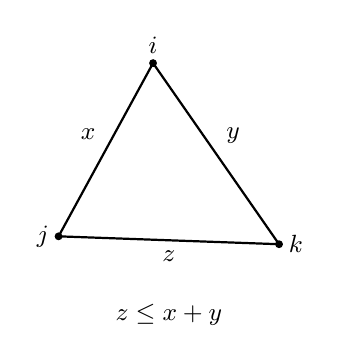
\begin{tikzpicture}[every node/.style={font=\small}]
      \coordinate (i) at (1.2,2.2); \coordinate (j) at (0,0); \coordinate (k) at (2.8,-0.1);
      \draw[thick] (i) -- node[above left] {$x$} (j) -- node[below] {$z$} (k) -- node[above right] {$y$} cycle;
      \foreach \p/\pos in {i/above, j/left, k/right} \fill (\p) circle (0.05) node[\pos] {$\p$};
      \node at (1.4,-1.0) {$z\leq x+y$};
    \end{tikzpicture}
    \caption{}
  \end{subfigure}\hfill
  \begin{subfigure}[b]{0.3\linewidth}
    \centering
    \begin{tikzpicture}[every node/.style={font=\small}, >=Stealth]
      \fill[blue!45] (-0.1,-0.1) rectangle (3.3,3.3);
      \pgfmathsetseed{5}
      \foreach \a in {0,...,7} \foreach \b in {0,...,7} {
        \pgfmathsetmacro{\v}{15+60*rnd}
        \fill[green!\v!teal!70!black] (0.4*\a,0.4*\b) rectangle ++(0.37,0.37);
      }
      % columns/rows: i=1, j=3, k=6 ; row index r at y = 0.4*(7-r)
      \foreach \lab/\c in {i/1, j/3, k/6} {
        \node[above] at (0.4*\c+0.18,3.3) {$\lab$};
        \node[left] at (-0.1,0.4*7-0.4*\c+0.18) {$\lab$};
      }
      \draw[very thick, red!80!black] (0.4*3,0.4*6) rectangle ++(0.37,0.37);
      \node[white, font=\scriptsize] at (0.4*3+0.18,0.4*6+0.18) {$ij$};
      \draw[very thick, orange] (0.4*6,0.4*6) rectangle ++(0.37,0.37);
      \node[white, font=\scriptsize] at (0.4*6+0.18,0.4*6+0.18) {$ik$};
      \draw[very thick, orange] (0.4*6,0.4*4) rectangle ++(0.37,0.37);
      \node[white, font=\scriptsize] at (0.4*6+0.18,0.4*4+0.18) {$jk$};
      \draw[->, thick, orange] (0.4*6,0.4*6+0.18) -- (0.4*3+0.4,0.4*6+0.18);
      \draw[->, thick, orange] (0.4*6,0.4*4+0.3) -- (0.4*3+0.4,0.4*6+0.05);
    \end{tikzpicture}
    \caption{}
  \end{subfigure}\hfill
  \begin{subfigure}[b]{0.36\linewidth}
    \centering
    \includegraphics[width=\linewidth]{triangle_violations.pdf}
    \caption{}
  \end{subfigure}
  \caption{(a) Three residues $i,j,k$ and the distances between them, which satisfy the triangle inequality. (b) In a triangle update, the entry $ij$ of the pair representation is updated from the entries $ik$ and $jk$, for every third residue $k$ (here for one $k$, and for the ``outgoing'' orientation). (c) Fraction of the triples of residues of an ideal 30-residue $\alpha$-helix whose distances violate the triangle inequality when each pairwise \Ca{} distance is perturbed by independent Gaussian noise (20 replicates per noise level). A long helix has many nearly collinear triples (in half of all triples the longest side is within 1\,\AA{} of the sum of the other two), so small independent errors already make the distances inconsistent. (a,b) after slides by M.~AlQuraishi and N.~Bouatta.}
  \label{fig:triangle}
\end{figure}

\paragraph{Triangle multiplicative updates.} Two gated linear maps of the pair representation give $\va_{ij}=\sigm(\mW^{A_1}\vz_{ij})\odot\mW^{A_2}\vz_{ij}$ and $\vc_{ij}=\sigm(\mW^{C_1}\vz_{ij})\odot\mW^{C_2}\vz_{ij}$, both in $\R^{D_t}$ (new maps, unrelated to those of the outer product mean), where $\odot$ is the elementwise product. The update ``using outgoing edges'' is
\begin{equation}
  \vz_{ij} \leftarrow \vz_{ij} + \vg_{ij}\odot\mW^O\LN\Big(\sum_{k=1}^R \va_{ik}\odot\vc_{jk}\Big), \qquad \vg_{ij} = \sigm(\mW^G\vz_{ij}),
  \label{eq:tri_mult}
\end{equation}
which combines the two edges leaving $i$ and $j$ towards each third residue $k$. The update ``using incoming edges'' replaces the sum by $\sum_k\va_{ki}\odot\vc_{kj}$. Both orientations are needed because the pair representation is not symmetric: $\vz_{ij}$ and $\vz_{ji}$ are different vectors. For each channel $d$, the sum $\sum_k a_{ik,d}\,c_{jk,d}$ is entry $ij$ of the matrix product $\mathbf{A}_d\mathbf{C}_d^\top$ of the $R\times R$ matrices of channel $d$, so the layer costs $O(R^3D_t)$. An intuition: if $\mathbf{A}_d$ and $\mathbf{C}_d$ were both the contact map, $\sum_k a_{ik}c_{jk}$ would count the residues in contact with both $i$ and $j$. Two residues with many common neighbours are likely to be close themselves, which is the kind of reasoning the triangle inequality supports.

\paragraph{Triangle self-attention.} Fix residue $i$ and view row $i$ of the pair representation, the edges $(i,1),\dots,(i,R)$, as a sequence. In triangle attention ``around the starting node'' edge $ij$ attends to edge $ik$, with a bias from the third edge $jk$,
\begin{equation}
  a^m_{ijk} = \softmax_k\left(\frac{\vq^{m\top}_{ij}\vk^m_{ik}}{\sqrt{P}} + b^m_{jk}\right), \qquad
  \vz_{ij} \leftarrow \vz_{ij} + \mW^O\operatorname{concat}_m\Big(\sum_{k=1}^R a^m_{ijk}\vv^m_{ik}\Big),
  \label{eq:tri_att}
\end{equation}
where queries, keys and values are linear maps of the pair representation, $\vq^m_{ij}=\mW^{Q,m}\vz_{ij}$ and so on, and $b^m_{jk}=\vw^{B,m\top}\vz_{jk}$. Triangle attention ``around the ending node'' does the same along columns: edge $ij$ attends to edge $kj$ with bias from $ki$. Each costs $O(R^3)$ scores per head, more than any other layer for long proteins. Triangle attention is the pair-representation analogue of row-wise attention with pair bias: in both, which other elements to attend to is informed by the pair representation.

\subsection{The Evoformer block}

Algorithm~\ref{alg:evoformer} lists the operations of one Evoformer block. Each is wrapped in a residual connection, so the block computes a sequence of additive updates to the two representations. The block is repeated 48 times with separate parameters, so information passes between the two tracks 48 times. The representations that come out are abstract: their channels have no predefined meaning, and although the pair representation is intended to encode geometry and to be approximately consistent with the triangle inequality, nothing in the architecture forces it to be. The geometry becomes explicit only in the structure module.

\begin{algorithm}[!htbp]
  \caption{One Evoformer block. Inputs are the MSA representation $\{\vm_{si}\}$ ($S\times R\times D_m$) and the pair representation $\{\vz_{ij}\}$ ($R\times R\times D_z$).}
  \label{alg:evoformer}
  \begin{algorithmic}[1]
    \State $\vm \gets \vm + \text{RowAttentionWithPairBias}(\vm,\vz)$ \Comment{\eqref{eq:row_attention}; pair $\to$ MSA}
    \State $\vm \gets \vm + \text{ColumnAttention}(\vm)$
    \State $\vm \gets \vm + \text{Transition}(\vm)$ \Comment{position-wise MLP}
    \State $\vz \gets \vz + \text{OuterProductMean}(\vm)$ \Comment{\eqref{eq:opm}; MSA $\to$ pair}
    \State $\vz \gets \vz + \text{TriangleMultiplicationOutgoing}(\vz)$ \Comment{\eqref{eq:tri_mult}}
    \State $\vz \gets \vz + \text{TriangleMultiplicationIncoming}(\vz)$
    \State $\vz \gets \vz + \text{TriangleAttentionStartingNode}(\vz)$ \Comment{\eqref{eq:tri_att}}
    \State $\vz \gets \vz + \text{TriangleAttentionEndingNode}(\vz)$
    \State $\vz \gets \vz + \text{Transition}(\vz)$
    \State \Return $\vm,\vz$
  \end{algorithmic}
\end{algorithm}

%======================================================================
\section{The structure module}
\label{sec:structure_module}
%======================================================================

The structure module receives the single representation $\vs_i\in\R^{D_s}$, for $i=1,\dots,R$, and the pair representation $\vz_{ij}$ from the last Evoformer block, and outputs the coordinates of every atom. It does so by placing each residue in space as a rigid body and refining the placement over eight blocks. This section describes how a residue's placement is represented, why the module must respect rotations and translations, and the attention layer that makes it do so.

\subsection{Backbone frames}

Fixing bond lengths and angles at their ideal values, the backbone atoms N, \Ca{} and C of a residue form a rigid triangle (Figure~\ref{fig:backbone}). Placing this triangle in space takes six numbers: three for its position and three for its orientation. AlphaFold represents the placement of residue $i$ as a \emph{frame}, or rigid transformation,
\begin{equation}
  T_i = (\mR_i,\vt_i), \qquad \mR_i\in\SO, \quad \vt_i\in\R^3,
\end{equation}
where $\vt_i$ is the position of the \Ca{} atom and $\mR_i$ is a rotation matrix, an element of the group $\SO=\{\mR\in\R^{3\times3}:\mR^\top\mR=\mI,\ \det\mR=1\}$ of rotations of three-dimensional space (Figure~\ref{fig:frame}). The columns of $\mR_i$ are the axes of a local coordinate system attached to the residue, written in global coordinates. A point with local coordinates $\vx\in\R^3$ has global coordinates
\begin{equation}
  T_i\circ\vx = \mR_i\vx + \vt_i ,
  \label{eq:frame_action}
\end{equation}
rotate first, then translate. The inverse maps global coordinates to local ones, subtracting the translation first and then undoing the rotation,
\begin{equation}
  T_i^{-1}\circ\vx = \mR_i^\top(\vx - \vt_i), \qquad T_i^{-1} = (\mR_i^\top,\,-\mR_i^\top\vt_i),
\end{equation}
using $\mR_i^{-1}=\mR_i^\top$. Composing two frames gives a frame, $T_a\circ T_b = (\mR_a\mR_b,\ \mR_a\vt_b+\vt_a)$, as can be checked by applying both sides to a point $\vx$: $T_a\circ(T_b\circ\vx)=\mR_a(\mR_b\vx+\vt_b)+\vt_a$. With these operations the set of frames is the group $\SE$ of rigid motions, the special Euclidean group. In the local frame, the backbone atoms of every residue have the same, idealized coordinates $\vx^{\text{N}}_{\text{loc}}$, $\vx^{\text{C}\alpha}_{\text{loc}}=\mathbf{0}$ and $\vx^{\text{C}}_{\text{loc}}$, so the global coordinates of the backbone of residue $i$ are $T_i\circ\vx^{\text{N}}_{\text{loc}}$, $\vt_i$ and $T_i\circ\vx^{\text{C}}_{\text{loc}}$.

Conversely, given the coordinates $\vx^{\text{N}}_i,\vx^{\text{C}\alpha}_i,\vx^{\text{C}}_i$ of a residue in an experimental structure, its frame is built by Gram--Schmidt orthogonalization. With $\vu_1=\vx^{\text{C}}_i-\vx^{\text{C}\alpha}_i$ and $\vu_2=\vx^{\text{N}}_i-\vx^{\text{C}\alpha}_i$,
\begin{equation}
  \ve_1 = \frac{\vu_1}{\|\vu_1\|}, \qquad
  \ve_2 = \frac{\vu_2-(\ve_1^\top\vu_2)\ve_1}{\|\vu_2-(\ve_1^\top\vu_2)\ve_1\|}, \qquad
  \ve_3 = \ve_1\times\ve_2, \qquad
  \mR_i = [\ve_1\ \ve_2\ \ve_3], \quad \vt_i = \vx^{\text{C}\alpha}_i .
  \label{eq:gram_schmidt}
\end{equation}
The vectors $\ve_1$ and $\ve_2$ are orthonormal and span the plane of the three atoms, and the cross product $\ve_3$ completes them to a right-handed basis, so $\det\mR_i=1$.

\begin{figure}[!htbp]
  \centering
  \begin{tikzpicture}[>=Stealth, every node/.style={font=\small}]
    % global axes
    \draw[->, thick] (0,0) -- (2.4,0) node[right] {$x$};
    \draw[->, thick] (0,0) -- (0,2.2) node[above] {$y$};
    \draw[->, thick] (0,0) -- (-1.1,-1.0) node[below left] {$z$};
    \node[below right] at (0,0) {global origin};
    % residue triangle
    \coordinate (CA) at (5.5,2.0); \coordinate (Cc) at (6.9,1.6); \coordinate (Nn) at (5.0,0.9);
    \fill[red!15, draw=red!70!black, thick] (Nn) -- (CA) -- (Cc) -- cycle;
    \foreach \p/\l/\pos in {CA/C$\alpha$/above, Cc/C/right, Nn/N/below left} \fill (\p) circle (0.06) node[\pos] {\l};
    % translation
    \draw[->, very thick, blue!70!black] (0,0) -- node[below right, pos=0.55] {$\vt_i$} (CA);
    % local axes
    \draw[->, thick, orange!90!black] (CA) -- ($(CA)!1.1cm!(Cc)$) node[above right] {$\ve_1$};
    \draw[->, thick, orange!90!black] (CA) -- ++(-0.45,-0.85) node[left] {$\ve_2$};
    \draw[->, thick, orange!90!black] (CA) -- ++(0.15,1.05) node[above] {$\ve_3$};
    \node[orange!70!black, align=left] at (9.2,2.3) {$\mR_i=[\ve_1\ \ve_2\ \ve_3]$\\ local axes in\\ global coordinates};
    \node at (8.6,0.5) {$T_i=(\mR_i,\vt_i)$};
  \end{tikzpicture}
  \caption{The frame of residue $i$. The translation $\vt_i$ is the position of the \Ca{} atom, and the columns of the rotation $\mR_i$ are the axes of a local coordinate system attached to the N--\Ca--C triangle, built from the atom positions by~\eqref{eq:gram_schmidt}. The axis $\ve_3$ points out of the plane of the triangle. After a slide by M.~AlQuraishi and N.~Bouatta.}
  \label{fig:frame}
\end{figure}

\subsection{The residue gas}

In a real protein the triangles are chained together: the C atom of residue $i$ is bonded to the N atom of residue $i+1$ at a distance of about 1.33\,\AA. Constraints like this are awkward for a neural network to impose exactly. AlphaFold does not impose them. It treats the protein as a \emph{residue gas}, a bag of $R$ independent triangles, each free to move and rotate, with $6R$ degrees of freedom in total. The network must learn that consecutive residues belong next to each other; at the end of training a loss term penalizes violated bond lengths and angles and clashes between atoms. Ignoring the chain makes every residue's update local and parallel, so that all parts of the structure can be refined at the same time rather than by propagating changes along the chain.

The structure module starts from what the authors call a \emph{black hole} initialization: every frame is the identity, $T_i=(\mI,\mathbf{0})$, so all residues sit at the origin with the same orientation (Figure~\ref{fig:residue_gas}a). Each of the eight blocks then moves and rotates every triangle a little, and by the last block the triangles should sit where the residues of the true structure are (Figure~\ref{fig:residue_gas}b).

\subsection{Invariance and equivariance}

A protein does not know where it is in space or which way it faces. If we rotate and translate the true structure by a global rigid motion $T_g=(\mR_g,\vt_g)$, every atom $\vx$ moves to $T_g\circ\vx$ and every frame $T_i$ to $T_g\circ T_i$, but it is the same structure. This places two requirements on the model.

A quantity computed from a structure, such as a loss or a distance, should be \emph{invariant}: $f(\{T_g\circ T_i\})=f(\{T_i\})$ for every $T_g\in\SE$. A map that updates a structure, such as one block $\varphi$ of the structure module, which takes frames $\{T_i\}$ to updated frames, should be \emph{equivariant}: it should commute with global motions,
\begin{equation}
  \varphi(\{T_g\circ T_i\}) = \{T_g\circ T'_i\}, \qquad\text{where } \{T'_i\}=\varphi(\{T_i\}).
  \label{eq:equivariance}
\end{equation}
In words, rotating the input and then updating gives the same result as updating and then rotating the output (Figure~\ref{fig:equivariance}). This is not automatic: a generic neural network applied to coordinates does not commute with rotations. It would have to learn the symmetry from data, by seeing structures in all orientations, and would still only approximate it.

The requirement is for $\SE$, rotations and translations, and not for the larger group $\mathrm{E}(3)$ that also contains reflections. A mirror image of a protein is a different molecule. Amino acids other than glycine are chiral, natural proteins are built from the L forms, and the $\alpha$-helix is right-handed; the mirror-image protein, built from D-amino acids, does not occur in nature and interacts differently with other chiral molecules. More generally in biochemistry, the two mirror-image forms of a chiral drug can have different effects. A structure predictor must therefore distinguish a structure from its mirror image.

The Evoformer raises none of these issues, because its representations contain no coordinates: the pair representation is invariant by construction, and template and recycled structures enter only through invariant features such as distances. The problem arises once frames are introduced in the structure module. AlphaFold makes each block equivariant through two components: an attention layer whose output is invariant to global motions, and an update rule that turns invariant features into equivariant frame updates.

\begin{figure}[!htbp]
  \centering
  \begin{tikzpicture}[>=Stealth, every node/.style={font=\small},
      rt/.style={draw=red!70!black, thick, fill=red!15},
      yt/.style={draw=yellow!60!black, thick, fill=yellow!30}]
    \newcommand{\ax}[1]{\draw[->, gray] #1 -- ++(1.0,0); \draw[->, gray] #1 -- ++(0,1.0); \draw[->, gray] #1 -- ++(-0.5,-0.45);}
    % (a) black hole
    \begin{scope}
      \ax{(0,0)}
      \foreach \d in {0,0.05,0.1,0.15} \draw[rt] (-0.4+\d,-0.2+\d) -- (0.1+\d,0.35+\d) -- (0.55+\d,-0.1+\d) -- cycle;
      \node at (0.3,-1.2) {(a) black hole initialization};
    \end{scope}
    % (b) residue gas
    \begin{scope}[xshift=4.8cm]
      \foreach \x/\y/\a in {-1.0/0.2/10, 0.0/0.7/-20, 0.9/0.0/35, 1.8/0.8/-5, 0.6/-0.7/60, -0.4/-0.6/-40} {
        \begin{scope}[shift={(\x,\y)}, rotate=\a]
          \draw[rt] (-0.3,-0.15) -- (0.05,0.25) -- (0.4,-0.1) -- cycle;
        \end{scope}
      }
      \node at (0.4,-1.2) {(b) residue gas};
    \end{scope}
    % (c) invariant point attention
    \begin{scope}[xshift=9.6cm]
      \foreach \x/\y/\a [count=\n] in {-1.2/-0.4/10, -0.2/-0.6/-15, 0.9/-0.5/25, 1.8/-0.3/-5} {
        \begin{scope}[shift={(\x,\y)}, rotate=\a]
          \draw[rt] (-0.3,-0.15) -- (0.05,0.25) -- (0.4,-0.1) -- cycle;
          \coordinate (k\n) at (0.05,0.6);
        \end{scope}
        \fill[red!70!black] (k\n) circle (0.06);
      }
      \begin{scope}[shift={(0.3,1.0)}, rotate=-10]
        \draw[yt] (-0.3,-0.15) -- (0.05,0.25) -- (0.4,-0.1) -- cycle;
        \coordinate (q) at (0.1,-0.45);
      \end{scope}
      \fill[yellow!50!black] (q) circle (0.06);
      \foreach \n in {1,...,4} \draw[gray] (q) -- (k\n);
      \node[yellow!40!black, font=\footnotesize] at (1.3,1.25) {residue $i$};
      \node at (0.3,-1.2) {(c) invariant point attention};
    \end{scope}
  \end{tikzpicture}
  \caption{(a) The structure module starts with every residue's triangle at the origin with the identity orientation. (b) Its blocks move each triangle independently; the residues are not explicitly chained (the residue gas). (c) In invariant point attention, residue $i$ (yellow) attends to residue $j$ (red) more when the query point it places in its own frame is close, in global space, to the key point that residue $j$ places in its frame. After slides by M.~AlQuraishi and N.~Bouatta.}
  \label{fig:residue_gas}
\end{figure}

\begin{figure}[!htbp]
  \centering
  \begin{tikzpicture}[>=Stealth, every node/.style={font=\small},
      rt/.style={draw=red!70!black, thick, fill=red!15},
      yt/.style={draw=yellow!60!black, thick, fill=yellow!30}]
    \newcommand{\gas}[2]{%
      \begin{scope}[shift={#1}, rotate=#2]
        \draw[->, gray] (0,0) -- (0.9,0); \draw[->, gray] (0,0) -- (0,0.9);
        \foreach \x/\y/\a in {0.1/0.15/0, 0.45/0.5/30, 0.75/0.1/-20} {
          \begin{scope}[shift={(\x,\y)}, rotate=\a] \draw[rt] (-0.15,-0.08) -- (0.02,0.12) -- (0.2,-0.05) -- cycle; \end{scope}
        }
      \end{scope}}
    \newcommand{\gasb}[2]{%
      \begin{scope}[shift={#1}, rotate=#2]
        \draw[->, gray] (0,0) -- (0.9,0); \draw[->, gray] (0,0) -- (0,0.9);
        \foreach \x/\y/\a in {0.25/0.25/40, 0.6/0.7/-10, 0.95/0.35/70} {
          \begin{scope}[shift={(\x,\y)}, rotate=\a] \draw[yt] (-0.15,-0.08) -- (0.02,0.12) -- (0.2,-0.05) -- cycle; \end{scope}
        }
      \end{scope}}
    \gas{(0,2.6)}{0}
    \gas{(5.2,2.4)}{35}
    \gasb{(0,0)}{0}
    \gasb{(5.2,-0.2)}{35}
    \node at (0.5,3.9) {$\{T_i\}$};
    \node at (5.3,3.9) {$\{T_g\circ T_i\}$};
    \node at (0.5,-0.55) {$\{T'_i\}$};
    \node at (5.3,-0.55) {$\{T_g\circ T'_i\}$};
    \draw[->, thick, teal!70!black] (1.6,3.0) -- node[above] {$T_g\in\SE$} (4.3,3.0);
    \draw[->, thick, teal!70!black] (1.6,0.4) -- node[below] {$T_g$} (4.4,0.4);
    \draw[->, thick, teal!70!black] (0.5,2.4) -- node[left] {$\varphi$} (0.5,1.3);
    \draw[->, thick, teal!70!black] (5.0,2.2) -- node[right] {$\varphi$} (5.0,1.3);
  \end{tikzpicture}
  \caption{Equivariance of a structure module block $\varphi$. Applying a global rotation and translation $T_g$ and then the block (right path) gives the same frames as applying the block and then $T_g$ (left and bottom path). After a slide by M.~AlQuraishi and N.~Bouatta.}
  \label{fig:equivariance}
\end{figure}

\subsection{Invariant point attention}

\emph{Invariant point attention} (IPA) updates the single representation using the single and pair representations and the current frames. It is attention over residues with three terms in the score. For head $m$, the first two are as in~\eqref{eq:row_attention}: an inner product of a query $\vq^m_i$ and key $\vk^m_j$ computed from $\vs_i$ and $\vs_j$, and a bias $b^m_{ij}$ projected from $\vz_{ij}$. Neither involves coordinates. The third is geometric. Each residue also produces $N_q$ query points $\vq^{mp}_i\in\R^3$ and key points $\vk^{mp}_j\in\R^3$, $p=1,\dots,N_q$, by linear maps of $\vs_i$, and these are interpreted as points in the residue's \emph{local} frame. Residue $i$ attends to residue $j$ more when its query points, placed in space by its frame, land close to the key points of residue $j$ placed by $j$'s frame,
\begin{equation}
  a^m_{ij} = \softmax_j\left( w_L\left( \frac{\vq^{m\top}_i\vk^m_j}{\sqrt{P}} + b^m_{ij} - \frac{\gamma^m w_C}{2}\sum_{p=1}^{N_q}\big\|T_i\circ\vq^{mp}_i - T_j\circ\vk^{mp}_j\big\|^2 \right)\right),
  \label{eq:ipa}
\end{equation}
where $\gamma^m>0$ is a learned weight per head and $w_L$, $w_C$ are fixed constants that keep the three terms on comparable scales. The squared distance enters with a minus sign, so nearby points increase the attention weight. In the published model there are $M=12$ heads and $N_q=4$ query points per head.

The output for residue $i$ combines three kinds of values with the same attention weights: scalar values $\vv^m_j$ computed from $\vs_j$, the pair representation $\vz_{ij}$, and $N_v$ value points $\vv^{mp}_j\in\R^3$ in the local frame of $j$. The value points are moved to global coordinates, averaged, and moved back into the local frame of $i$,
\begin{equation}
  \vo^{m}_i=\sum_j a^m_{ij}\vv^m_j, \qquad
  \tilde\vo^{m}_i=\sum_j a^m_{ij}\vz_{ij}, \qquad
  \vo^{mp}_i = T_i^{-1}\circ\Big(\sum_{j=1}^R a^m_{ij}\, T_j\circ\vv^{mp}_j\Big),
  \label{eq:ipa_out}
\end{equation}
and $\vs_i$ is updated by a linear map of the concatenation of all these outputs and the norms $\|\vo^{mp}_i\|$.

\paragraph{Why the output is invariant.} Apply a global motion to all frames, $T_j\mapsto T_g\circ T_j$ for every $j$, while $\vs$ and $\vz$, which carry no coordinates, are unchanged. The local points $\vq^{mp}_i$, $\vk^{mp}_j$ and $\vv^{mp}_j$ are computed from $\vs$ and so are unchanged too. In the score,
\begin{equation}
  (T_g\circ T_i)\circ\vq - (T_g\circ T_j)\circ\vk = \big(\mR_g(T_i\circ\vq)+\vt_g\big) - \big(\mR_g(T_j\circ\vk)+\vt_g\big) = \mR_g\big(T_i\circ\vq - T_j\circ\vk\big),
\end{equation}
the translation cancels, and the rotation does not change the norm, $\|\mR_g\vu\|^2=\vu^\top\mR_g^\top\mR_g\vu=\|\vu\|^2$. So every $a^m_{ij}$ is unchanged. For the point output, using $\sum_j a^m_{ij}=1$,
\begin{align}
  (T_g\circ T_i)^{-1}\circ\Big(\sum_j a^m_{ij}\,(T_g\circ T_j)\circ\vv^{mp}_j\Big)
  &= T_i^{-1}\circ T_g^{-1}\circ\Big(\mR_g\sum_j a^m_{ij}\,T_j\circ\vv^{mp}_j + \vt_g\Big) \nonumber\\
  &= T_i^{-1}\circ\Big(\sum_j a^m_{ij}\,T_j\circ\vv^{mp}_j\Big) = \vo^{mp}_i ,
\end{align}
since $T_g^{-1}\circ(\mR_g\vu+\vt_g)=\vu$. The weights summing to one is what lets the translation pass through the average. All outputs, and therefore the updated $\vs_i$, are invariant. The geometric term gives the network a way to reason about which residues are near which in the current structure, while its output stays independent of the global frame.

\subsection{Updating the frames}

After IPA and a transition MLP, a linear layer predicts from each $\vs_i$ an update to frame $i$: a vector $\boldsymbol{\kappa}_i\in\R^3$ that defines a rotation through the unit quaternion $(1,\kappa_{i1},\kappa_{i2},\kappa_{i3})/\sqrt{1+\|\boldsymbol{\kappa}_i\|^2}$, and a translation $\vt^{\text{upd}}_i\in\R^3$. For a unit quaternion $(\eta_0,\eta_1,\eta_2,\eta_3)$ the rotation matrix is
\begin{equation}
  \mR = \begin{pmatrix}
    \eta_0^2+\eta_1^2-\eta_2^2-\eta_3^2 & 2(\eta_1\eta_2-\eta_0\eta_3) & 2(\eta_1\eta_3+\eta_0\eta_2)\\
    2(\eta_1\eta_2+\eta_0\eta_3) & \eta_0^2-\eta_1^2+\eta_2^2-\eta_3^2 & 2(\eta_2\eta_3-\eta_0\eta_1)\\
    2(\eta_1\eta_3-\eta_0\eta_2) & 2(\eta_2\eta_3+\eta_0\eta_1) & \eta_0^2-\eta_1^2-\eta_2^2+\eta_3^2
  \end{pmatrix},
\end{equation}
which is a valid rotation for any $\boldsymbol{\kappa}_i$, and close to the identity when $\boldsymbol{\kappa}_i$ is small. Fixing the first component to one keeps each update a modest rotation. The update is composed on the right,
\begin{equation}
  T_i \leftarrow T_i\circ T^{\text{upd}}_i, \qquad T^{\text{upd}}_i=(\mR^{\text{upd}}_i,\vt^{\text{upd}}_i),
  \label{eq:frame_update}
\end{equation}
so that it is expressed in the residue's local frame: $\vt^{\text{upd}}_i$ is a step along the residue's own axes.

\paragraph{Why the update is equivariant.} Because $\vs_i$ is invariant, so is $T^{\text{upd}}_i$. If all frames are first moved to $T_g\circ T_i$, the updated frame is $(T_g\circ T_i)\circ T^{\text{upd}}_i = T_g\circ(T_i\circ T^{\text{upd}}_i)$ by associativity, which is the global motion applied to the frame updated without it. This is exactly the equivariance~\eqref{eq:equivariance}. Composing on the left, $T^{\text{upd}}_i\circ T_i$, would not work, because an update predicted from invariant features would then move every residue along the same global axes whatever the orientation of the protein.

\subsection{Side chains}

The frames place the backbone. For the side chains, a small residual network predicts seven torsion angles per residue from $\vs_i$: the backbone torsions $\omega$, $\phi$, $\psi$ and the side-chain torsions $\chi_1,\dots,\chi_4$ (unused ones are ignored). An angle lives on a circle, not on the real line: $359^\circ$ and $1^\circ$ are close. Each angle is therefore predicted as an unnormalized vector in $\R^2$ and normalized onto the unit circle, giving $(\cos\theta,\sin\theta)$ without a discontinuity. A pair of angles such as $(\phi,\psi)$ lives on a torus, the product of two circles, on which the Ramachandran plot is naturally drawn. Given the frames and torsion angles, the coordinates of all side-chain atoms follow from idealized bond geometry: each side chain is a chain of rigid groups, each rotated about a bond by one torsion angle relative to the previous group. Since the torsions are computed from the invariant $\vs_i$ and the atoms are placed relative to the frame $T_i$, the full-atom structure is equivariant too.

\subsection{Iterative refinement and recycling}

Algorithm~\ref{alg:structure_module} summarizes the structure module. The eight blocks share their weights, so the module applies the same update repeatedly, moving the residues step by step from the black hole towards the structure, much as an iterative algorithm would. Unlike the hidden layers of a typical network, the state after each block is already a structure, which is what makes the intermediate losses of the next section possible. Recycling wraps the whole network in a second loop (Algorithm~\ref{alg:recycling}), so that inference is a nested loop of refinement.

\begin{algorithm}[!htbp]
  \caption{Structure module (simplified). $\vs_i\in\R^{D_s}$ and $\vz_{ij}\in\R^{D_z}$ come from the Evoformer.}
  \label{alg:structure_module}
  \begin{algorithmic}[1]
    \State $T_i\gets(\mI,\mathbf{0})$ for all $i$ \Comment{black hole initialization}
    \For{$\ell=1,\dots,8$} \Comment{shared weights}
      \State $\vs \gets \vs + \text{IPA}(\vs,\vz,\{T_i\})$ \Comment{\eqref{eq:ipa}--\eqref{eq:ipa_out}; invariant}
      \State $\vs \gets \vs + \text{Transition}(\vs)$
      \State $T_i \gets T_i\circ\text{BackboneUpdate}(\vs_i)$ for all $i$ \Comment{\eqref{eq:frame_update}; equivariant}
      \State predict torsion angles from $\vs_i$; compute backbone loss terms for this block
    \EndFor
    \State compute all atom coordinates from $\{T_i\}$ and the torsion angles
  \end{algorithmic}
\end{algorithm}

\begin{algorithm}[!htbp]
  \caption{AlphaFold~2 inference with recycling.}
  \label{alg:recycling}
  \begin{algorithmic}[1]
    \State search databases for the MSA and templates of the input sequence
    \State set the recycled features to zero
    \For{$c=0,1,2,3$} \Comment{three recycling iterations after the first pass}
      \State embed MSA, templates and pair features; add the recycled features
      \State $(\vm,\vz)\gets$ 48 Evoformer blocks (Algorithm~\ref{alg:evoformer}); $\vs_i\gets$ linear map of $\vm_{1i}$
      \State structure, confidence $\gets$ structure module (Algorithm~\ref{alg:structure_module})
      \State recycled features $\gets$ first MSA row $\vm_{1\cdot}$, pair representation $\vz$, distances in the predicted structure
    \EndFor
  \end{algorithmic}
\end{algorithm}

%======================================================================
\section{Training}
\label{sec:training}
%======================================================================

AlphaFold~2 is trained end to end, from MSA and templates to atom coordinates, on structures from the PDB. The loss has several terms. The main one compares predicted and true structures; the others supervise intermediate outputs and auxiliary predictions.

\subsection{Frame aligned point error}

Comparing two structures requires care, because the prediction lives in an arbitrary global frame. The usual metric, the root mean square deviation (RMSD) of atom positions, first superimposes the prediction on the truth by the rotation and translation that minimize it. A single global superposition is dominated by the largest errors: if two domains are each predicted well but their relative orientation is wrong, no superposition fits both. An alternative that needs no superposition is the distance RMSD (dRMSD), which compares all pairwise distances, $\sqrt{\text{mean}_{i<j}(d_{ij}-d^{\text{true}}_{ij})^2}$. Distances are invariant to rotations and translations, but also to reflections, so a mirror image of the true structure has a dRMSD of zero.

The \emph{frame aligned point error} (FAPE) avoids both problems by aligning on every residue in turn. For each frame $i$ and each atom $j$, it expresses the atom in the residue's local frame, in both the predicted and the true structure,
\begin{equation}
  \vx_{ij} = T_i^{-1}\circ\vx_j, \qquad \vx^{\text{true}}_{ij} = (T_i^{\text{true}})^{-1}\circ\vx^{\text{true}}_j ,
\end{equation}
where $\vx_j\in\R^3$ is the predicted global position of atom $j$, and the true frames $T^{\text{true}}_i$ are built from the experimental coordinates by~\eqref{eq:gram_schmidt}. The error for the pair is
\begin{equation}
  d_{ij} = \sqrt{\big\|\vx_{ij} - \vx^{\text{true}}_{ij}\big\|^2 + \varepsilon},
\end{equation}
and the loss averages a clamped version over all $N_{\text{frames}}$ frames and $N_{\text{atoms}}$ atoms,
\begin{equation}
  \mathcal{L}_{\text{FAPE}} = \frac{1}{Z}\,\frac{1}{N_{\text{frames}}N_{\text{atoms}}}\sum_{i=1}^{N_{\text{frames}}}\sum_{j=1}^{N_{\text{atoms}}}\min\left(d_{\text{clamp}},\,d_{ij}\right),
  \label{eq:fape}
\end{equation}
with $d_{\text{clamp}}=10$\,\AA, $Z=10$\,\AA{} a length scale that makes the loss unitless, and $\varepsilon=10^{-4}$\,\AA$^2$ (Figure~\ref{fig:fape}a). The small $\varepsilon$ inside the square root makes $d_{ij}$ differentiable everywhere: the Euclidean norm $\|\vu\|$ has gradient $\vu/\|\vu\|$, which has unit length however small $\vu$ is and is undefined at $\vu=\mathbf{0}$, while $\sqrt{\|\vu\|^2+\varepsilon}$ is smooth and equals $\|\vu\|$ to within a small fraction of an \aa{}ngstr\"om. Clamping stops gross errors, such as a misplaced domain, from dominating the gradient, so that the loss rewards getting local structure right; in most training examples the clamp is applied.

\paragraph{Invariance.} Apply a global motion $T_g$ to the predicted structure, so that $T_i\mapsto T_g\circ T_i$ and $\vx_j\mapsto T_g\circ\vx_j$. Then
\begin{equation}
  (T_g\circ T_i)^{-1}\circ(T_g\circ\vx_j) = T_i^{-1}\circ T_g^{-1}\circ T_g\circ\vx_j = T_i^{-1}\circ\vx_j = \vx_{ij},
\end{equation}
so FAPE is unchanged, and the same holds for the true structure. No superposition step is needed: each frame defines its own alignment, and FAPE averages the error over $N_{\text{frames}}$ different alignments.

\paragraph{Reflections.} FAPE does distinguish a structure from its mirror image. Let $\mM$ be a reflection, an orthogonal matrix with $\det\mM=-1$, for example $\operatorname{diag}(1,1,-1)$, and suppose the predicted atoms are the reflected true atoms, $\vx_j=\mM\vx^{\text{true}}_j$. In the Gram--Schmidt construction~\eqref{eq:gram_schmidt}, $\vu_1$ and $\vu_2$ become $\mM\vu_1$ and $\mM\vu_2$, so $\ve_1\mapsto\mM\ve_1$ and $\ve_2\mapsto\mM\ve_2$. For an orthogonal $\mM$, $(\mM\va)\times(\mM\vc)=\det(\mM)\,\mM(\va\times\vc)$, so $\ve_3\mapsto-\mM\ve_3$. The predicted frame is therefore $\mR_i=\mM\mR^{\text{true}}_i\mathbf{D}$ with $\mathbf{D}=\operatorname{diag}(1,1,-1)$ and $\vt_i=\mM\vt^{\text{true}}_i$, and the local coordinates are
\begin{equation}
  \vx_{ij} = \mathbf{D}\mR^{\text{true}\top}_i\mM^\top\mM\big(\vx^{\text{true}}_j-\vt^{\text{true}}_i\big) = \mathbf{D}\,\vx^{\text{true}}_{ij}.
\end{equation}
The third local coordinate, the height of atom $j$ above the plane of residue $i$, changes sign, so $d_{ij}\approx2|(\vx^{\text{true}}_{ij})_3|$, which is zero only for atoms in the plane of residue $i$. Figure~\ref{fig:fape}b confirms this on an ideal $\alpha$-helix. Its mirror image, a left-handed helix, has a dRMSD of zero, while its FAPE is 8.3\,\AA{} (before division by $Z$) and its superposed RMSD 3.2\,\AA. The figure also shows that FAPE responds more steeply than RMSD to errors in the backbone torsion angles: a small change of a residue's orientation moves distant atoms far in that residue's frame.

\begin{figure}[!htbp]
  \centering
  \begin{subfigure}[b]{0.44\linewidth}
    \centering
    \begin{tikzpicture}[>=Stealth, every node/.style={font=\small},
        rt/.style={draw=red!70!black, thick, fill=red!15}]
      % experimental
      \begin{scope}
        \draw[rt] (0,0) -- (0.4,0.5) -- (0.85,0.05) -- cycle;
        \draw[->, gray] (0.4,0.5) -- ++(0.7,0) ; \draw[->, gray] (0.4,0.5) -- ++(0,0.7);
        \fill[blue!60!black] (1.2,1.6) circle (0.07);
        \draw[dashed, blue!60!black] (0.4,0.5) -- (1.2,1.6);
        \node[blue!60!black, right] at (1.25,1.6) {$\vx^{\text{true}}_{ij}$};
        \node at (0.6,-0.5) {true, frame $i$};
      \end{scope}
      \begin{scope}[xshift=3.0cm]
        \draw[rt] (0,0) -- (0.4,0.5) -- (0.85,0.05) -- cycle;
        \draw[->, gray] (0.4,0.5) -- ++(0.7,0) ; \draw[->, gray] (0.4,0.5) -- ++(0,0.7);
        \fill[orange!80!black] (1.45,1.35) circle (0.07);
        \fill[blue!60!black, opacity=0.4] (1.2,1.6) circle (0.07);
        \draw[dashed, orange!80!black] (0.4,0.5) -- (1.45,1.35);
        \draw[<->, thick] (1.2,1.6) -- (1.45,1.35) node[right] {$d_{ij}$};
        \node[orange!80!black, right] at (1.5,1.0) {$\vx_{ij}$};
        \node at (0.6,-0.5) {predicted, frame $i$};
      \end{scope}
      \node[align=center, font=\footnotesize] at (2.2,-1.25) {atom $j$ in the frame of residue $i$,\\ compared after aligning frame $i$};
    \end{tikzpicture}
    \caption{}
  \end{subfigure}\hfill
  \begin{subfigure}[b]{0.54\linewidth}
    \includegraphics[width=\linewidth]{fape_vs_rmsd.pdf}
    \caption{}
  \end{subfigure}
  \caption{(a) FAPE expresses each atom $j$ in the local frame of each residue $i$, in the true and in the predicted structure, and measures the distance $d_{ij}$ between the two. (b) Errors of perturbed copies of an ideal 30-residue $\alpha$-helix, in which every $\phi$ and $\psi$ angle is perturbed by Gaussian noise and the backbone rebuilt with ideal geometry, as a function of the noise standard deviation (mean $\pm$ one s.d.\ over 30 replicates; each copy is also randomly rotated). FAPE is reported in \AA{} before division by $Z$; RMSD is the \Ca{} RMSD after optimal superposition; dRMSD compares \Ca{} distances. Dashed lines show the values for the mirror image of the helix: its dRMSD is zero.}
  \label{fig:fape}
\end{figure}

\paragraph{Which frames and atoms.} The final FAPE uses all atoms and the frames of all rigid groups, backbone and side chain. Some side chains are symmetric, for example the two oxygens of aspartate are chemically equivalent, and the true structure is relabelled to whichever naming better matches the prediction before the loss is computed.

\subsection{Auxiliary and intermediate losses}

The other terms are as follows.

\begin{itemize}
  \item \emph{Intermediate structure loss} $\mathcal{L}_{\text{aux}}$. Because the state after each block of the structure module is a structure, the loss can be computed there too. $\mathcal{L}_{\text{aux}}$ averages, over the eight blocks, a backbone-only FAPE and a loss on the predicted torsion angles. Normally a loss is computed only at the output of a network, since the hidden layers are abstract; here every block is pushed to produce a good structure, and the authors' ablations show that this helps.
  \item \emph{Distogram loss} $\mathcal{L}_{\text{dist}}$. A linear layer on the symmetrized pair representation $\vz_{ij}+\vz_{ji}$ predicts a distribution $p_{ij}(b)$ over 64 bins $b$ of the distance between the C$\beta$ atoms of residues $i$ and $j$ (\Ca{} for glycine), from 2 to 22\,\AA. The loss is the cross-entropy $-\frac{1}{R^2}\sum_{i,j}\sum_b y_{ij}(b)\log p_{ij}(b)$, where $y_{ij}(b)=1$ if the true distance falls in bin $b$ and zero otherwise. This is the AlphaFold~1 objective, kept as an auxiliary signal that supervises the pair representation directly.
  \item \emph{Masked MSA loss} $\mathcal{L}_{\text{MSA}}$. Before the MSA enters the network, 15\% of its entries are selected and corrupted: most are replaced by a mask token, and the rest by a random amino acid, by an amino acid sampled from the column's frequency profile, or left unchanged. A linear layer on the final MSA representation predicts the original residue at the selected entries, with a cross-entropy loss. This is the masked language modelling objective of BERT~\citep{devlin2019}: to fill in a masked residue the network must learn the dependencies between columns and between homologs, the coevolution signal of Section~\ref{sec:evolution}.
  \item \emph{Confidence loss} $\mathcal{L}_{\text{conf}}$, described next.
\end{itemize}

\subsection{Predicting confidence}

AlphaFold~2 predicts how accurate each part of its prediction is. The target is the \emph{local distance difference test} (lDDT)~\citep{mariani2013}, a superposition-free score. For residue $i$, take all residues $j$ whose \Ca{} atoms are within 15\,\AA{} of residue $i$'s in the true structure. For each threshold $\tau\in\{0.5,1,2,4\}$\,\AA, compute the fraction of these $j$ for which the predicted and true distances agree to within $\tau$, $|d_{ij}-d^{\text{true}}_{ij}|<\tau$. The lDDT-\Ca{} of residue $i$ is the average of the four fractions, times 100. It measures how well the local environment of each residue is reproduced, between 0 and 100.

A small network on the final single representation $\vs_i$ predicts a distribution over 50 bins of lDDT for each residue, trained by cross-entropy against the lDDT of the predicted structure computed during training. The mean of the predicted distribution is the \emph{pLDDT}, the per-residue confidence used to colour structures (Figure~\ref{fig:af2_arch}). A related head on the pair representation predicts the expected error in the position of residue $j$ when the predicted and true structures are aligned on the frame of residue $i$, which indicates whether the relative placement of two domains is reliable.

It may seem surprising that a network can predict its own errors, since neural networks are often poorly calibrated. One reason it works here is that the uncertainty has biological sources the network can learn to recognize: low pLDDT often marks intrinsically disordered regions, and shallow MSAs give less reliable predictions.

\subsection{The full objective}

The loss for the main stage of training combines the terms,
\begin{equation}
  \mathcal{L} = 0.5\,\mathcal{L}_{\text{FAPE}} + 0.5\,\mathcal{L}_{\text{aux}} + 0.3\,\mathcal{L}_{\text{dist}} + 2.0\,\mathcal{L}_{\text{MSA}} + 0.01\,\mathcal{L}_{\text{conf}} .
  \label{eq:full_loss}
\end{equation}
A final fine-tuning stage adds a penalty $\mathcal{L}_{\text{viol}}$ on violations of bond lengths, bond angles and steric clashes, which is how the chain constraints ignored by the residue gas are eventually enforced, and a small loss for predicting which atoms are experimentally resolved. Training used structures from the PDB and, in addition, about 350,000 high-confidence predictions made by an earlier version of the model for sequences without known structures, a form of self-distillation that increased accuracy.

\subsection{Performance and what matters}

In the CASP14 blind assessment in 2020, AlphaFold~2 predicted protein backbones with a median error of about 1\,\AA{} (\Ca{} RMSD over 95\% of residues), compared with about 3\,\AA{} for the next best method, and was often competitive with experimental structures~\citep{jumper2021}. Its authors' ablation studies show that most of the bespoke components contribute: removing invariant point attention, the triangle updates, recycling, the intermediate losses or the masked MSA objective each lowers accuracy. The MSA matters a great deal. Accuracy falls sharply for proteins whose alignments contain fewer than about 30 effective sequences, so orphan proteins and rapidly evolving families remain difficult.

AlphaFold's predictions for over 200 million proteins have been made public~\citep{varadi2022}. Later models build on the same ideas. RoseTTAFold~\citep{baek2021} uses three coupled tracks, for sequence, pairs and coordinates. ESMFold~\citep{lin2023} replaces the MSA with the representations of a protein language model trained by masked language modelling on millions of sequences, which have learned coevolutionary information implicitly. AlphaFold~3~\citep{abramson2024} keeps a pair-centric trunk with triangle updates but replaces the structure module with a diffusion model over atom coordinates, which extends prediction to complexes of proteins with nucleic acids, small molecules and ions.

%======================================================================
\section{Summary}
%======================================================================

\begin{itemize}
  \item AlphaFold~2 predicts the 3D coordinates of all atoms of a protein from its sequence, together with a per-residue confidence. It is trained end to end on experimental structures from the PDB.
  \item Much of its information comes from evolution. A multiple sequence alignment of homologs reveals conserved positions and pairs of positions that co-evolve, which tend to be in contact in the structure. Coevolution statistics such as mutual information must be corrected for phylogeny and indirect correlations.
  \item The Evoformer updates an MSA representation ($S\times R\times D_m$) and a pair representation ($R\times R\times D_z$) over 48 blocks. Axial attention along rows and columns keeps the cost of attending over the MSA manageable. The pair representation biases row attention (pair to MSA); the outer product mean, a learned version of the pair frequency table, updates the pair representation (MSA to pair). Triangle multiplicative updates and triangle attention update each pair entry $ij$ from the entries $ik$ and $jk$, so the network can learn the consistency that the triangle inequality demands of distances.
  \item The structure module represents each residue as a rigid frame $T_i=(\mR_i,\vt_i)$, ignores the chain (the residue gas), and starts with all frames at the origin. Invariant point attention adds to the attention score a term that depends on distances between points in global space, so its output is invariant to global rotations and translations; frame updates predicted from invariant features and composed on the right make each block equivariant. Reflections are not a symmetry, because proteins are chiral.
  \item The main loss, FAPE, compares predicted and true atom positions in the local frame of every residue, which is invariant to global motions without superposition and, unlike distance-based losses, distinguishes mirror images. Auxiliary losses supervise every structure module block, the distogram and a masked MSA objective, and a confidence head learns to predict the lDDT of its own prediction.
\end{itemize}

%======================================================================
\section*{Exercises}
%======================================================================

\begin{enumerate}
  \item Show that for one-hot inputs $\vm_{si}=\ve_{x_{si}}\in\{0,1\}^q$ the outer product mean~\eqref{eq:opm} equals $\mW^A\mF_{ij}\mW^{C\top}$, where $\mF_{ij}$ is the pair frequency table~\eqref{eq:msa_freqs}. Can a single outer product mean layer followed by a linear map compute the mutual information between columns $i$ and $j$? What does the network need in addition?
  \item For an MSA with $S$ sequences and $R$ residues, count the attention scores computed by full attention over all $SR$ entries and by one row-wise plus one column-wise attention layer. For $R=384$, how large can $S$ be before axial attention computes more scores than full attention over the $R^2$ pair entries with triangle attention, which computes $2R^3$ scores per head?
  \item Prove that triangle attention around the starting node~\eqref{eq:tri_att} is equivariant to permutations of the residues: if the residues are reordered by a permutation $\pi$, so that $\vz'_{ij}=\vz_{\pi(i)\pi(j)}$, the output is reordered in the same way.
  \item Show that the frames with composition $T_a\circ T_b=(\mR_a\mR_b,\mR_a\vt_b+\vt_a)$ form a group: find the identity, verify the inverse $T^{-1}=(\mR^\top,-\mR^\top\vt)$, and show that composition is associative.
  \item Show that IPA would not be invariant if the attention weights did not sum to one over $j$, by computing the point output~\eqref{eq:ipa_out} after a global translation $\vt_g$ with unnormalized weights.
  \item Modify \texttt{scripts/make\_figures.py} to compute the lDDT-\Ca{} of the perturbed helices in Figure~\ref{fig:fape}b and of the mirror image. Is lDDT invariant to reflections? What does that imply for using pLDDT to detect a mirror-image prediction?
  \item Show that the Gram--Schmidt construction~\eqref{eq:gram_schmidt} applied to the atoms $T_g\circ\vx^{\text{N}}_i$, $T_g\circ\vx^{\text{C}\alpha}_i$, $T_g\circ\vx^{\text{C}}_i$ gives the frame $T_g\circ T_i$, for any $T_g\in\SE$.
\end{enumerate}

